\chapter{Saturn} \label{chapter:sat}
\section{Overview}
Saturn is the main co-ordinator service which acts as a bridge between the client facing service and the other backend services (i.e. Olivia and Classifier). It handles all the front-end HTTP requests and data that is being sent in either via x-www-form or JSON. Saturn has been through a number of evolutions due to the various stages of agile development. During initial development stage, Saturn was the only back-end service where every major computations were performed locally. At present, all complex computational operations are allocated to two remote services which are linked to Saturn. Below is the list of tasks that is handled by Saturn:

\begin{enumerate}
      \item Communicates with Olivia for extracting attributes from image tile
           \item  Communicates with Classifier to classify or reclassify the data
          \item Communicates with Classifier to get list of all data that belongs to certain theme
          \item   Communicates with Classifier to reset, delete and clear the data set
      \item Manages the `Discover’ sweep from the GUI
\end{enumerate}
\section{Design}
During the first iteration, the whole back-end system design was a single modular system based on Monolithic architecture. All the feature extraction and classification tasks were handled internally, by the single saturn server. Later, the design architecture was changed to micro-services where each major task is now allocated to remote services for computing. 

Saturn has dedicated modules for each server with specialised methods defined within it, to carry out certain functionality. For instance, it has an Olivia module which has a method called ``get\_all\_attr\_vecs(image\_list)” which takes a list of image URLs as parameter. When the method is invoked, it will then send the list to Olivia server for extracting the image’s attributes and returns a dictionary of URL as key with its corresponding attributes as values.
\begin{figure}[H]
    \centering
    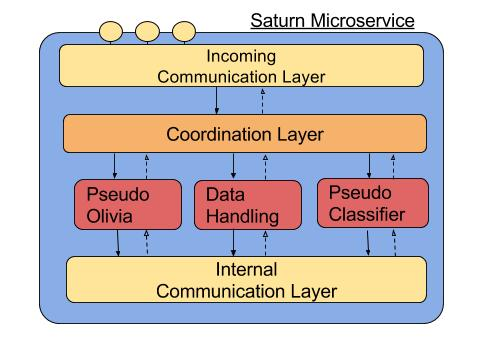
\includegraphics{figs/9/scl}
    \caption{Saturn Internal Communication Architecture}
    \label{fig:sat:scl}
\end{figure}
Figure \ref{fig:sat:scl} shows the internal structure of Saturn server where incoming request are handled by Incoming communication layer and transferred to Coordination layer. Coordination layer is linked to Olivia and Classifier module which are responsible for communicating with remote servers. Internal Communication layer handles all the data that is being communicated services `internal’ to the back-end.
\subsection{Data Handling}
As the main interface to the back end services, Saturn must have more complex data manipulation to handle a range of error inputs. It can accept x-wwww-form and JSON formatted data. When the server gets the request from front-end GUI, it will extract relevant provided data and repurpose it for use with the next services; removing any redundant or unnecessary pieces of data. This data is then converted to JSON to send to the next service. Having a structured style helps to maintain uniformity throughout the application system and avoids any kind of confusion during communication.

Saturn server has a list of endpoints that respond to certain tasks such as: finding them; classifying data; extracting attributes; clearing data; resetting data and downloading data. Certain endpoints merely act as routers, passing the message on. For example the saturn/clear endpoint triggers olivia/clear and classifier/clear. 
The key function within Saturn is the Feature Finder, or the `discover’ sweep from the GUI perspective. This service extensively uses the other services to perform its own computation to determine the class of each individual image tiles based on the returned data from Classifier. It has method that determines the class of the specific tiles based on its probability value. As mentioned earlier, each tile is computed nine times using the NSEW technique in Olivia (defined in section \ref{section:nsew}) and classified in Classifier. Using that returned data, Saturn assigns probability value to each tile requested based on their given feature type. Saturn will choose the class which has the highest probability value from among all nine tiles to determine class of single image tile.

\subsection{Error Handling}
Saturn ensures a uniformity in its returns by catching all the exceptions. Connection errors and connection timeout exceptions are two of the more frequently observed errors due to the issue . It also handles all the error message that is being passed from remote servers. It analyses the returned data and in case of any error found, it will include appropriate error messages to be transmitted to the front end. For instance, if Olivia failed to download and extract some of the image tiles attributes, it will first check if there is any failed image that is being returned. If yes then it will include the error message and returns the data to the front-end server in JSON format. This makes it much easier for client applications to consume saturn's data and encouraging them to communicate with saturn, ensuring the correct flow of service usage.

\subsection{Global Persistence vs Local Persistence}
Initial system design was to implement a global persistence system which acts as a main body for storing and communicating the data. However, this system design made other servers depended on Saturn as they will have to request for data every time to perform any task. This proved to be an ineffective way to program an application using micro-service architecture. Now Saturn doesn’t hold any data by itself. Each remote server store their data locally which Saturn can access by making data request. The reason for such design change was to make each service or server self-sufficient to perform the given task.
\section{Evaluation}
Saturn has a good communication architecture that can handle all the request from front-end GUI. It follows a structured messaging style to communicate the data which prevents any occurrence of human error when passing the data. Having a dedicated endpoint for each task makes it easier for front-end server to invoke the right endpoint. By tidying data and offering the feature finder as a macro function encourages clients to use Saturn rather than incorrectly using the other micro services. Overall Saturn performance is very good when it comes to coordinating task and communicating between the remote servers.